
\section{\texorpdfstring{$\mathcal{D}$}{D} 上\trMetric{} \texorpdfstring{$d$}{d} 与%
\texorpdfstring{$C^{0}$}{C0}-\trMetric{}的比较}
\label{sec:metric-c0-comparison}

\hzsync{theorem}{9}%
\hzsync{lemma}{8}%
\hzsync{definition}{6}%
\hzsync{equation}{26}%

为了理解 5.1 节中在 $\mathcal{D}$ 上引入的\trMetric{} $d$，将它同一些更为%
熟悉的\trMetric{}作比较是有益的。例如人们可以问：一个同\trIdentityMap{}%
$C^{0}$-接近的\trSymplectic{}映射，能否由一个 $C^{0}$-小的%
\trHamiltonianFunction{}生成？情形未必如此，我们将借助 $\R^{2}$ 中的一个%
例子来表明这一点。我们将构造一列 $\psi_{n}\in\mathcal{D}$，满足
\begin{align}
\lvert\psi_{n}-\id\rvert_{C^{0}}\quad&\longrightarrow\quad 0\notag\\
d(\psi_{n},\id)\quad&\longrightarrow\quad\infty.
\label{eq:divergence-example}
\end{align}
我们取如下定义的诸\trHamiltonianFunction{} $H_{n}\in\mathcal{H}$：
\[
H_{n}(x,y)=\frac{1}{n}f_{n}(x)\chi_{n}(x,y)\qquad\text{于}\ \R^{2}.
\]
这里 $f_{n}\in C^{\infty}(\R)$ 满足：当 $0\leq x\leq n^{2}$ 时%
$f_{n}(x)=x$，其图形如图 5.7 所示：

\noindent\begin{minipage}{\linewidth}
\centering
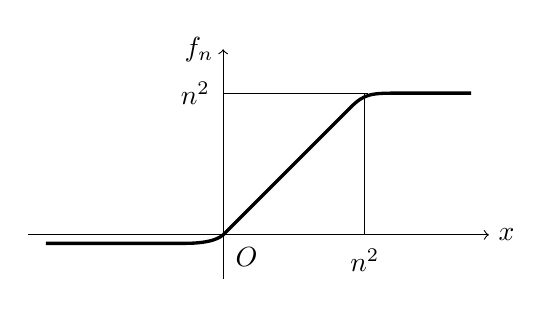
\begin{tikzpicture}[scale=0.9]
  \draw[->] (-2.75,0) -- (3.75,0) node[right] {$x$};
  \draw[->] (0,-0.62) -- (0,2.62) node[left] {$f_{n}$};
  \node[anchor=north west] at (0.04,-0.04) {$O$};
  \draw[thin] (0,2) -- (2.05,2);
  \draw[thin] (2,0) -- (2,2);
  \node[anchor=east] at (-0.05,2) {$n^{2}$};
  \node[anchor=north] at (2,-0.06) {$n^{2}$};
  \draw[very thick] (-2.5,-0.12) -- (-0.55,-0.12)
    .. controls (-0.14,-0.12) and (-0.04,-0.03) .. (0,0)
    -- (1.8,1.8)
    .. controls (2.0,2.0) and (2.1,2.0) .. (2.5,2.0)
    -- (3.5,2.0);
\end{tikzpicture}

图 5.7
\end{minipage}

此外，$\chi_{n}\in C^{\infty}_{c}\bigl(\R^{2}\bigr)$ 是一个光滑的\trCutoff{}%
函数，它在由 $0\leq x\leq n^{2}$、$0\leq y\leq\frac{2}{n}$ 给出的\trDomain{}%
上等于 $1$，并缓慢递减使得 $\lvert\nabla\chi_{n}\rvert\leq\frac{1}{n^{2}}$：

\noindent\begin{minipage}{\linewidth}
\centering
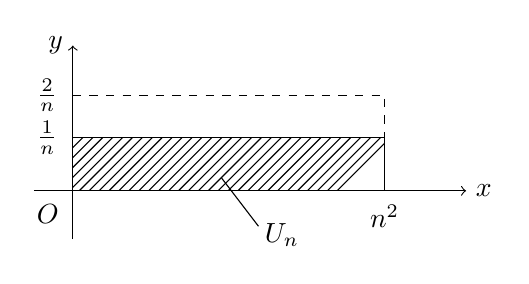
\begin{tikzpicture}[scale=0.9]
  \draw[->] (-0.55,0) -- (5.55,0) node[right] {$x$};
  \draw[->] (0,-0.68) -- (0,2.05) node[left] {$y$};
  \node[anchor=north east] at (-0.06,-0.06) {$O$};
  \begin{scope}
    \clip (0,0) rectangle (4.4,0.75);
    \foreach \i in {0,...,32} \draw[thin] (0.14*\i-0.75,0) -- (0.14*\i,0.75);
  \end{scope}
  \draw[thin] (0,0) rectangle (4.4,0.75);
  \draw[dashed,thin] (0,1.35) -- (4.4,1.35) -- (4.4,0.75);
  \node[anchor=east] at (-0.08,1.35) {$\frac{2}{n}$};
  \node[anchor=east] at (-0.08,0.75) {$\frac{1}{n}$};
  \node[anchor=north] at (4.4,-0.06) {$n^{2}$};
  \draw[thin] (2.62,-0.5) -- (2.1,0.18);%
  \node at (2.95,-0.62) {$U_{n}$};
\end{tikzpicture}

图 5.8
\end{minipage}

设 $\psi_{n}=\varphi_{H_{n}}\in\mathcal{D}$ 为由 $H_{n}$ 生成的诸映射。由于%
图 5.8 中的集合 $U_{n}$ 被 $\psi_{n}$ 从其自身挪开，我们便可以依据%
\cref{thm:energy-dominates-capacity}%
作出估计 $d(\psi_{n},\id)=E(\psi_{n})\geq c_{0}(U_{n})=n$。另一方面，%
$\lvert\psi_{n}-\id\rvert_{C^{0}}\leq\frac{C}{n}$，论断%
\eqref{eq:divergence-example} 即得证。

对这个例子而言，诸映射 $\psi_{n}$ 的\trSupport{}的直径不断增长是重要的。%
的确，若使诸\trSupport{}保持一致\trBounded，这样的例子便不存在。这可由%
下述归于 H.~\trHofer{} [117] 的\trEstimate{}看出：

\begin{theorem}\label{thm:c0-comparison}
对每一对 $\varphi,\psi\in\mathcal{D}$，
\[
d(\varphi,\psi)\ \leq\ C\ \operatorname{diameter\,supp}\bigl(\varphi\psi^{-1}\bigr)%
\ \lvert\varphi-\psi\rvert_{C^{0}}
\]
其中 $C$ 是一个常数且 $C\leq128$。
\end{theorem}

本节的其余部分将用于这条把内蕴\trMetric{} $d$ 同 $C^{0}$-\trMetric{}加以%
比较的陈述的证明。我们需要一些技术性的准备，并从一个\trhDefinition{}开始。%
下文的记号涉及\trSymplecticSplitting{} $\R^{2n}=\R^{2}\oplus\dots\oplus\R^{2}$%
与坐标 $(x_{1},y_{1},\dots,x_{n},y_{n})$。若 $a\in\R$，我们将以%
$\{x_{1}=a\}$ 记\trHyperplane{}%
$\bigl\{(x,y)\in\R^{2n}\ \bigm|\ x_{1}=a\bigr\}$。

\begin{definition}\label{def:properly-separated}
以 $S_{1},\dots,S_{k}$ 记 $\R^{2n}$ 的任意子集。若对\trBounded{}子集的每一种%
取法 $A_{j}\subset S_{j}$，都存在一个\trMapping{} $\tau\in\mathcal{D}$ 与数%
$a_{1}<a_{2}<\dots<a_{k-1}$，使得诸集合 $\tau(A_{j})$ 位于%
$\R^{2n}\setminus\bigcup_{j=1}^{k-1}\{x_{1}=a_{j}\}$ 的不同%
\trConnectedComponent{}之中，则称它们是\textbf{\trProperlySeparated}（properly %
 separated）的。将诸集合重新标记之后，我们可以假定 $\tau(A_{j})$ 位于%
$\tau(A_{j+1})$ 的左侧：
\begin{center}
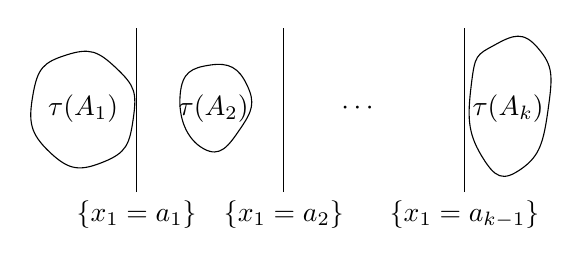
\begin{tikzpicture}[scale=0.85]
  \draw[thin] (1.4,-1.05) -- (1.4,1.4);
  \draw[thin] (3.6,-1.05) -- (3.6,1.4);
  \draw[thin] (6.3,-1.05) -- (6.3,1.4);
  \draw[smooth cycle,tension=1] plot coordinates{(-0.15,0.4) (0.35,1.0) (1.1,0.8)
    (1.35,0.05) (0.9,-0.6) (0.1,-0.45)};
  \draw[smooth cycle,tension=1] plot coordinates{(2.05,0.4) (2.5,0.85) (3.05,0.55)
    (2.95,-0.1) (2.4,-0.4)};
  \draw[smooth cycle,tension=1] plot coordinates{(6.4,0.55) (6.75,1.15) (7.4,1.1)
    (7.55,0.2) (7.15,-0.7) (6.55,-0.5)};
  \node at (0.6,0.2) {$\tau(A_{1})$};
  \node at (2.55,0.2) {$\tau(A_{2})$};
  \node at (4.7,0.2) {$\cdots$};
  \node at (6.95,0.2) {$\tau(A_{k})$};
  \node at (1.4,-1.38) {$\{x_{1}=a_{1}\}$};
  \node at (3.6,-1.38) {$\{x_{1}=a_{2}\}$};
  \node at (6.3,-1.38) {$\{x_{1}=a_{k-1}\}$};
\end{tikzpicture}
\end{center}
\end{definition}

\begin{lemma}\label{lem:translation-separation}
设诸集合 $S_{1},\dots,S_{k}$ \trBounded{}且已被平行的\trHyperplane{}正常%
分离。那么，给定 $R>0$，存在一个\trMapping{} $\tau=\tau_{R}\in\mathcal{D}$%
与向量 $v_{1},v_{2},\dots,v_{k}\in\R^{2n}$，其中 $v_{1}=0$，满足
\[
\tau(x)=x+v_{j}\qquad\text{若}\quad x\in S_{j}
\]
对一切 $1\leq j\leq k$ 成立，并且
\[
\operatorname{dist}\bigl(\tau(S_{j}),\tau(S_{i})\bigr)\ \geq\ R\qquad\text{若}%
\quad i\neq j.
\]
\end{lemma}

\begin{proof}
取 $0=\alpha_{1}<\alpha_{2}<\dots<\alpha_{k}$，我们引入向量
\[
v_{j}=\alpha_{j}e_{1}\qquad\in\R^{2n},
\]
其中 $e_{1}=(1,0,0,\dots\,0)$，以及平移后的集合
\[
S_{j}^{t}:=S_{j}+tv_{j}.
\]
对每个 $t\geq0$，这些集合彼此不交且被诸\trHyperplane{}分离。当%
$t\to\infty$ 时，彼此间的\trDistance{}趋于无穷。如下定义\trMapping
\[
H\ :\ \bigcup_{t\geq0}\{t\}\times\Bigl(\bigcup_{j=1}^{k}S_{j}^{t}\Bigr)%
\longrightarrow\R
\]
当 $(x,y)\in S_{j}^{t}$ 时令 $H(t,x,y)=\alpha_{j}y_{1}$。我们可以把 $H$ 视为%
$\R\times\R^{2n}$ 上某个\trSmooth{}\trHamiltonianFunction{}的限制，后者在%
空间变量上具有\trCompactSupport，而 $t$ 则局限于一个\trCompact{}区间内。%
若取 $\alpha_{j}=R(j-1)$，则时间-$t$映射 $\varphi_{H}^{t}$ 在每个集合%
$S_{j}$ 上的作用如同一个\trTranslation{} $S_{j}\cdot t=S_{j}+t\alpha_{j}e_{1}$。%
于是诸集合 $S_{j}\cdot t$ 之间的\trDistance{}至少为 $tR$，由此即证得该%
\trhLemma。
\end{proof}

\begin{lemma}\label{lem:energy-separated-product}
设 $\psi_{1},\psi_{2},\dots,\psi_{k}\in\mathcal{D}$ 的诸\trSupport{}正常%
分离。则
\[
E(\psi_{1}\psi_{2}\cdots\psi_{k})\ \leq\ 2\max_{j}E(\psi_{j}).
\]
注意，这些映射必可交换。
\end{lemma}

\begin{proof}
由于\trEnergy{} $E$ 在\trConjugate{}之下\trInvariant，我们可以假定诸%
$\psi_{j}$ 的\trSupport{}已被平行的\trHyperplane{}分离。先验地，我们不能%
假定生成诸\trHamiltonianFunction{}具有互不相交的\trSupport。因此我们使用%
一个技巧。设 $\psi_{j}=\varphi_{H_{j}}$，并把\trSupport{}记为%
$S_{j}=\operatorname{supp}(\psi_{j})$。选取 $R>0$ 使得
\[
\operatorname{supp}(H_{j})\ \subset\ [0,1]\times B_{R}(x_{j}^{*})
\]
其中 $x_{j}^{*}\in S_{j}$。现在选取向量 $v_{j}$，使得诸集合%
$B_{R}(S_{j}+v_{j})$ 互不相交。若 $\tau\in\mathcal{D}$ 是由%
\cref{lem:translation-separation}所保证的、与诸 $S_{j}$ 相伴的那个%
\trMapping，我们便令 $\hat{\psi}_{j}=\tau\psi_{j}\tau^{-1}$，并发现
\[
E(\psi_{1}\psi_{2}\cdots\psi_{k})=E(\hat{\psi}_{1}\hat{\psi}_{2}\cdots\hat{\psi}_{k}).
\]
由构造知 $\operatorname{supp}(\hat{\psi}_{j})=\tau(S_{j})=S_{j}+v_{j}$。现在%
注意，奇迹般地有
\[
\hat{\psi}_{j}(x)\ =\ \tau\psi_{j}\tau^{-1}(x)\ =\ \psi_{j}(x-v_{j})+v_{j}%
\ =\ \tau_{j}\psi_{j}\tau_{j}^{-1}(x)
\]
对一切 $x\in\R^{2n}$ 成立，其中\trTranslation{} $\tau_{j}(x)=x+v_{j}$。于是，%
依据\trHamiltonianVectorField{}的\trTransformationLaw，
\[
\hat{\psi}_{j}=\varphi_{\hat{H}_{j}}\qquad\text{其中}\quad \hat{H}_{j}(t,x)=H_{j}(t,x-v_{j}).
\]
由构造知诸 $\operatorname{supp}(\hat{H}_{j})$ 现在彼此不交，从而
\[
\hat{\psi}_{1}\hat{\psi}_{2}\cdots\hat{\psi}_{k}=\varphi_{\hat{H}}
\]
其中 $\hat{H}=\hat{H}_{1}+\hat{H}_{2}+\dots+\hat{H}_{k}$。给定%
$\varepsilon>0$，我们选取 $H_{j}$ 使得 $\lVert H_{j}\rVert\leq E(\psi_{j})+\varepsilon$，%
于是
\[
E(\psi_{1}\psi_{2}\cdots\psi_{k})=E(\varphi_{\hat{H}})\ \leq\ \lVert\hat{H}\rVert.
\]
按定义，
\[
\lVert\hat{H}\rVert\ =\ \int_{0}^{1}\Bigl(\sup_{x}\hat{H}_{t}-\inf_{x}\hat{H}_{t}\Bigr)dt,
\]
而由于诸 $\hat{H}_{j}$ 的\trSupport{}互不相交，我们有
\[
\lVert\hat{H}\rVert\ \leq\ 2\max_{j}\int_{0}^{1}\Bigl(\sup_{x}\hat{H}_{j}-\inf_{x}\hat{H}_{j}\Bigr)dt\ =\ 2\max_{j}\lVert\hat{H}_{j}\rVert\ \leq\ 2\max_{j}E(\psi_{j})+2\varepsilon.
\]
这对每个 $\varepsilon>0$ 都成立，该\trhLemma{}即得证。
\end{proof}

为了下文之用，引入\trDisplacementEnergy{}的一个加细是有益的。若%
$S\subset\R^{2n}$ 是任意子集，我们定义其\textbf{正常\trDisplacementEnergy{}}%
（proper displacement energy）$e_{p}(S)$ 为
\begin{align*}
e_{p}(S)\ =\ \inf\Bigl\{\,a>0\ \Bigm|\ &\text{对每个\trBounded{}子集}\ A\subset S\\
&\text{存在}\ \psi\in\mathcal{D}\ \text{满足}\ E(\psi)\leq a\ \text{且}\\
&\ A\ \text{与}\ \psi(A)\ \text{\trProperlySeparated}\,\Bigr\}.
\end{align*}
如前一节中那样，可以验证：$e_{p}$ 是 $\R^{2n}$ 中诸集合的一个特殊%
\trCapacity，并且它还满足 $e_{p}(B(1))=\pi=e_{p}(Z(1))$。一个令人惊讶的%
观察是：映射 $\psi\in\mathcal{D}$ 的\trEnergy{}，可以通过为用一个%
\trHamiltonianFunction{}生成该映射所需的最小\trSupport{}的正常%
\trDisplacementEnergy{}来估计。这是 J.C.~\trSikorav{}在 [198] 中发现的：

\begin{theorem}[J.C.~\trSikorav]\label{thm:sikorav-estimate}
若 $H\in\mathcal{H}$ 满足 $\operatorname{supp}(H)\subset[0,1]\times U$，则
\[
E(\varphi_{H})\ \leq\ 16\,e_{p}(U).
\]
\end{theorem}

\begin{proof}
以 $\varphi_{H}^{t}$ 记\trMapping{} $\varphi_{H}$ 的时间演化。给定%
$\varepsilon>0$，我们取 $N$ 充分大，使得由
\[
\psi_{k}=\varphi_{H}^{t_{k}}\ ,\qquad\text{其中}\ \ t_{k}=\frac{k}{N}\ ,\quad 0\leq k\leq N
\]
定义的诸映射 $\psi_{k}$ 满足
\begin{align*}
\psi_{0}\ &=\ \id\ ,\qquad\ \psi_{N}=\varphi_{H}\\
\operatorname{supp}(\psi_{k})\ &\subset\ S\subset U\ ,\qquad 0\leq k\leq N\\
d(\psi_{k},\psi_{k+1})\ &<\ \varepsilon\ ,\qquad 0\leq k\leq N-1.
\end{align*}
这里 $S\subset\R^{2n}$ 是 $U$ 的一个\trBounded{}子集。按 $e_{p}$ 的定义，%
存在 $\varphi\in\mathcal{D}$ 使得 $S$ 与 $\varphi(S)$ \trProperlySeparated，并且
\[
E(\varphi)\ \leq\ e_{p}(S)\ +\ \varepsilon\ \leq\ e_{p}(U)\ +\ \varepsilon.
\]
接下来我们对 $0\leq j\leq2N$ 构造一列特殊的映射 $\varphi_{j}\in\mathcal{D}$。%
若 $j=0,1$，我们令 $\varphi_{0}=\id$ 与 $\varphi_{1}=\varphi$。为了定义%
$\varphi_{2}$，我们先按\cref{lem:translation-separation}之证明中的方式选取%
一个\trMapping{} $\sigma_{2}\in\mathcal{D}$，它对 $s\in S$ 满足
\[
\sigma_{2}(s)=s\ ,\qquad \sigma_{2}\bigl(\varphi(s)\bigr)=\varphi(s)+v_{2}
\]
其中 $v_{2}\in\R^{2n}$ 为某一向量。令 $\varphi_{2}=\sigma_{2}\varphi\sigma_{2}^{-1}$，%
则对 $s\in S$ 有 $\varphi_{2}(s)=\sigma_{2}(\varphi(s))=\varphi(s)+v_{2}$。%
类似地，我们按
\[
\varphi_{j}=\sigma_{j}\varphi\sigma_{j}^{-1}\ ,\qquad 2\leq j\leq2N
\]
构造出全部映射 $\varphi_{j}$，并如此选取平移向量 $v_{j}$，使得由
\[
S_{j}=\varphi_{j}(S)\ ,\qquad 0\leq j\leq2N
\]
定义的集合序列 $S_{j}$ 互不相交且两两\trProperlySeparated。现在定义映射%
$\alpha_{j},\beta_{k}\in\mathcal{D}$ 如下：
\begin{align*}
\alpha_{j}\ &=\ \varphi_{2j-1}\psi_{j}\varphi_{2j-1}^{-1}\ ,\qquad 1\leq j\leq N\\
\beta_{k}\ &=\ \varphi_{2k}\psi_{k}^{-1}\varphi_{2k}^{-1}\ ,\qquad 0\leq k\leq N
\end{align*}
我们便看到
\begin{align*}
\operatorname{supp}(\alpha_{j})\ &\subset\ S_{2j-1}\ ,\qquad 1\leq j\leq N\\
\operatorname{supp}(\beta_{k})\ &\subset\ S_{2k}\ ,\qquad 0\leq k\leq N.
\end{align*}
由构造知诸\trSupport{}彼此不交，因此 $\alpha_{1},\dots,\alpha_{N},\beta_{0},\beta_{1}\dots\beta_{N}$%
中的任何两个映射都可交换。由于 $\beta_{N}=\varphi_{2N}\varphi_{H}^{-1}\varphi_{2N}^{-1}$%
\footnote{原书印作 $\varphi_{2N}\varphi_{H}\varphi_{2N}^{-1}$，依 $\beta_{k}$ 之定义%
疑为 $\varphi_{2N}\varphi_{H}^{-1}\varphi_{2N}^{-1}$ 之误，此处径改。——译者注}%
且 $\beta_{0}=\id$，我们可以利用诸映射的可交换性并计算
\begin{align*}
E(\varphi_{H})\ &=\ E(\beta_{N})\\
&=\ E\Bigl(\beta_{N}\Bigl(\prod_{k=0}^{N-1}\alpha_{k+1}\beta_{k}\Bigr)\Bigl(\prod_{k=0}^{N-1}\alpha_{k+1}\beta_{k}\Bigr)^{-1}\Bigr)\\
&=\ E\Bigl(\Bigl(\prod_{k=1}^{N}\alpha_{k}\beta_{k}\Bigr)\Bigl(\prod_{k=0}^{N-1}\alpha_{k+1}\beta_{k}\Bigr)^{-1}\Bigr)\\
&\leq\ 2\max_{1\leq k\leq N}E(\alpha_{k}\beta_{k})\ +\ 2\max_{0\leq k\leq N-1}E(\alpha_{k+1}\beta_{k}),
\end{align*}
其中我们用到了\cref{lem:energy-separated-product}。注意到
\[
\alpha_{k}\beta_{k}=\varphi_{2k-1}\bigl(\psi_{k}\varphi_{2k-1}^{-1}\varphi_{2k}\psi_{k}^{-1}\bigr)\varphi_{2k}^{-1}
\]
并回忆诸映射 $\varphi_{j}$ 都与 $\varphi$ 共轭，我们可以估计
\[
E(\alpha_{k}\beta_{k})\ \leq\ 4E(\varphi)\ \leq\ 4e_{p}(U)+4\varepsilon.
\]
类似地，利用
\[
\alpha_{k+1}\beta_{k}=\varphi_{2k+1}\bigl(\psi_{k+1}\psi_{k}^{-1}\bigr)\bigl(\psi_{k}\varphi_{2k+1}^{-1}\varphi_{2k}\psi_{k}^{-1}\bigr)\varphi_{2k}^{-1}
\]
我们发现
\begin{align*}
E(\alpha_{k+1}\beta_{k})\ &\leq\ 4E(\varphi)\ +\ d(\psi_{k},\psi_{k+1})\\
&\leq\ 4e_{p}(U)\ +\ 4\varepsilon\ +\ \varepsilon.
\end{align*}
总结起来我们得到 $E(\varphi_{H})\leq16e_{p}(U)+18\varepsilon$，而由于%
$\varepsilon>0$ 是任意的，\trSikorav{}定理的证明即告完成。
\end{proof}

\trSikorav{}估计的如下局部化形式，对\cref{thm:c0-comparison}的证明将是%
至关重要的。

\begin{lemma}\label{lem:sikorav-localization}
设 $\psi\in\mathcal{D}$，$\psi\neq\id$，并设 $\delta>\lvert\psi-\id\rvert_{C^{0}}$。%
对每个满足 $Q\cap\operatorname{supp}(\psi)\neq\varnothing$ 的\trOpenSet{}%
$Q\subset\R^{2n}$，存在一个 $\varphi\in\mathcal{D}$ 满足
\begin{align*}
\text{(i)}\qquad& \varphi\big|_{Q}=\psi\big|_{Q}\\
\text{(ii)}\qquad& \operatorname{supp}(\varphi)\ \subset\ U\\
\text{(iii)}\qquad& E(\varphi)\ \leq\ 16\,e_{p}(U),
\end{align*}
其中 $U=B_{\delta}(Q)\cap C$。这里 $C$ 是 $\operatorname{supp}(\psi)$ 的%
\textbf{\trConvexHull}（convex hull），而 $B_{\delta}(Q)=\bigl\{\,x\ \bigm|\ %
\operatorname{dist}(x,Q)<\delta\,\bigr\}$。
\end{lemma}

\begin{proof}
按定义，存在一条连接\trIdentityMap{}与 $\psi$ 的\trSmooth{}\trHomotopy{}%
$\psi^{t}$（$0\leq t\leq1$）。选取 $x_{0}\in Q\cap\operatorname{int\,supp}(\psi)$，%
我们可以找到一个 $R>0$ 使得
\begin{equation}\label{eq:homotopy-support-ball}
\operatorname{supp}(\psi^{t})\ \subset\ B_{R}(x_{0})\ ,\qquad 0\leq t\leq1.
\end{equation}
现在对 $0\leq s<1$ 与 $0\leq t\leq1$ 如下定义双参数族%
$\psi^{t}_{s}\in\mathcal{D}$：
\[
\psi^{t}_{s}(x)\ =\ sx_{0}+(1-s)\psi^{t}\Bigl(x_{0}+\frac{x-x_{0}}{1-s}\Bigr).
\]
易于验证
\begin{align}
\operatorname{supp}(\psi^{t}_{s})\ &\ \subset\ B_{(1-s)R}(x_{0})\label{eq:family-support}\\
\operatorname{supp}(\psi^{1}_{s})\ &\ \subset\ C.\label{eq:family-endpoint-support}
\end{align}
我们可以固定 $s_{0}\in(0,1)$ 使得
\begin{equation}\label{eq:ball-inside-QC}
B_{(1-s_{0})R}(x_{0})\ \subset\ Q\cap C,
\end{equation}
并如下定义一条连接\trIdentityMap{}与 $\psi$ 的新\trHomotopy{}%
$\varphi^{\tau}\in\mathcal{D}$（$0\leq\tau\leq1$）：
\[
\varphi^{\tau}=\psi^{t(\tau)}_{s(\tau)},
\]
其中\trSmooth{}函数 $t(\tau)$ 与 $s(\tau)$ 的选取使得曲线%
$\Gamma(\tau):=\bigl(t(\tau),s(\tau)\bigr)\subset\R^{2}$ 呈如下形状：

\noindent\begin{minipage}{\linewidth}
\centering
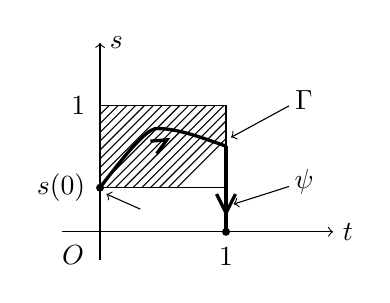
\begin{tikzpicture}[scale=1.6]
  \draw[->] (-0.3,0) -- (1.85,0) node[right] {$t$};
  \draw[->] (0,-0.22) -- (0,1.5) node[right] {$s$};
  \node[anchor=north east] at (-0.05,-0.03) {$O$};
  \begin{scope}
    \clip (0,0.35) rectangle (1,1);
    \foreach \i in {0,...,18} \draw[thin] (0.07*\i-0.65,0.35) -- (0.07*\i,1);
  \end{scope}
  \draw[thin] (0,0.35) rectangle (1,1);
  \draw[very thick] (0,0.35) .. controls (0.3,0.75) and (0.4,0.82) .. (0.45,0.82)
        .. controls (0.62,0.82) and (0.8,0.75) .. (1,0.68);
  \draw[very thick] (0.40,0.72) -- (0.53,0.73) -- (0.45,0.62);%
  \draw[very thick] (1,0.68) -- (1,0);
  \draw[very thick] (0.925,0.30) -- (1,0.15) -- (1.075,0.30);%
  \fill (0,0.35) circle (0.9pt);%
  \fill (1,0) circle (0.9pt);%
  \node[anchor=east] at (-0.04,0.35) {$s(0)$};
  \node[anchor=east] at (-0.04,1) {$1$};
  \node[anchor=north] at (1,-0.05) {$1$};
  \node at (1.62,1.05) {$\Gamma$};
  \draw[->] (1.5,1.0) -- (1.04,0.75);%
  \node at (0.32,0.1) {$\id$};
  \draw[->] (0.32,0.18) -- (0.05,0.3);%
  \node at (1.62,0.4) {$\psi$};
  \draw[->] (1.5,0.36) -- (1.06,0.22);%
\end{tikzpicture}

图 5.9
\end{minipage}

这里，曲线 $\Gamma$ 在 $0\leq\tau\leq\frac{1}{2}$ 时跑在带阴影的区域内，%
在 $\frac{1}{2}\leq\tau\leq1$ 时跑在竖直段上。于是，由%
\eqref{eq:family-support}、\eqref{eq:family-endpoint-support} 与%
\eqref{eq:ball-inside-QC} 可知：对一切 $0\leq\tau\leq1$ 都有%
$\operatorname{supp}(\varphi^{\tau})\subset C$，而当 $0\leq\tau\leq\frac{1}{2}$%
时 $\operatorname{supp}(\varphi^{\tau})\subset Q\cap C$。此外，当%
$\frac{1}{2}\leq\tau\leq1$ 时%
$\lvert\varphi^{\tau}-\id\rvert_{C^{0}}\leq\bigl(1-s(\tau)\bigr)\lvert\psi-\id\rvert_{C^{0}}$，%
这易于验证。从而
\begin{equation}\label{eq:phi-tau-Q}
\varphi^{\tau}(Q)\ \subset\ B_{d}(Q)\ ,\qquad 0\leq\tau\leq1
\end{equation}
其中 $d:=\lvert\psi-\id\rvert_{C^{0}}$。由于 $\operatorname{supp}(\varphi^{\tau})\subset C$%
且 $C$ 是凸的，这一\trHomotopy{}由一个\trHamiltonianFunction{}%
$F\in\mathcal{H}$ 生成：$\varphi^{\tau}=\varphi^{\tau}_{F}$，其\trSupport{}%
含于 $[0,1]\times C$。将此函数光滑地截断，我们便找到一个新的%
\trHamiltonianFunction{} $K$，它满足
\begin{align*}
K\big|_{B_{d}(Q)}\ &=\ F\big|_{B_{d}(Q)}\\
\operatorname{supp}(K)\ &\subset\ [0,1]\times B_{\delta}(Q).
\end{align*}
依据 \eqref{eq:phi-tau-Q}，我们对诸\trTimeOneMap{}得出%
$\varphi_{K}\big|_{Q}=\varphi_{F}\big|_{Q}=\psi\big|_{Q}$。此外，%
$\operatorname{supp}(K)\subset\bigl([0,1]\times B_{\delta}(Q)\bigr)\cap\operatorname{supp}(F)\subset[0,1]\times\bigl(B_{\delta}(Q)\cap C\bigr)$，%
从而 $\operatorname{supp}(\varphi_{K})\subset B_{\delta}(Q)\cap C$。我们可以%
应用\trSikorav{}定理并得到%
$E(\varphi_{K})\leq16\,e_{p}\bigl(B_{\delta}(Q)\cap C\bigr)$。令%
$\varphi=\varphi_{K}\in\mathcal{D}$，该\trhLemma{}即得证。
\end{proof}

我们还需要\trSikorav{}定理的另一个推论。

\begin{lemma}\label{lem:energy-box}
设 $\psi\in\mathcal{D}$ 且 $\operatorname{supp}(\psi)\subset U$。若%
$U=(a_{1},a_{2})\times(b_{1},b_{2})\oplus\R^{2n-2}$，则
\[
E(\psi)\ \leq\ 16(a_{2}-a_{1})(b_{2}-b_{1}).
\]
\end{lemma}

\begin{proof}
由于 $U$ 是凸的，我们仿照上述证明的第一部分构造一个\trHamiltonianFunction{}%
$H\in\mathcal{H}$，它满足 $\operatorname{supp}(H)\subset[0,1]\times U$ 并生成%
$\psi=\varphi_{H}$。仿照\cref{cor:ball-cylinder-pi}
之证明进行论证，易于验证 $e_{p}(U)=(a_{2}-a_{1})(b_{2}-b_{1})$，从而该%
\trhLemma{}就是上文\trSikorav{}定理的一个推论。
\end{proof}

\begin{proof}[\cref*{thm:c0-comparison}的证明]
我们考虑满足 $\psi\neq\id$ 的 $\psi\in\mathcal{D}$，并选取
\[
\delta>d=\lvert\psi-\id\rvert_{C^{0}}.
\]
由 $a_{0}=0$ 与 $a_{k+1}=a_{k}+2\delta$ 定义序列 $a_{j}$，我们令
\[
Q_{k}=\bigl[(a_{k}-\varepsilon,a_{k}+\varepsilon)\times\R\bigr]\oplus\R^{2n-2}
\]
其中 $0<\varepsilon<(\delta-d)$。由于 $\operatorname{supp}(\psi)$ 是%
\trCompact{}的，指标集
\[
I=\Bigl\{\,k\ \Bigm|\ Q_{k}\cap\operatorname{supp}(\psi)\neq\varnothing\Bigr\}
\]
是一个有限集。现在选取 $d<\delta_{1}<(\delta-\varepsilon)$。依据局部化的%
\cref{lem:sikorav-localization}，对每个 $k\in I$ 我们可以找到一个映射%
$\varphi_{k}\in\mathcal{D}$ 满足
\begin{align*}
\text{(i)}\qquad& \varphi_{k}\big|_{Q_{k}}=\psi\big|_{Q_{k}}\\
\text{(ii)}\qquad& \operatorname{supp}(\varphi_{k})\ \subset\ U_{k}\\
\text{(iii)}\qquad& E(\varphi_{k})\ \leq\ 16\,e_{p}(U_{k})
\end{align*}
其中 $U_{k}=B_{\delta_{1}}(Q_{k})\cap\text{\trConvexHull}\bigl(\operatorname{supp}(\psi)\bigr)$。%
由于 $B_{\delta_{1}}(Q_{k})=(a_{k}-\varepsilon-\delta_{1},a_{k}+\varepsilon+\delta_{1})\times\R^{2n-1}$%
且 $2(\varepsilon+\delta_{1})<2\delta$，这些集合是\trProperlySeparated{}的，从而诸%
$\operatorname{supp}(\varphi_{k})$ 亦然。简记
\[
R:=\operatorname{diameter\,supp}\ \psi,
\]
我们可以找到一列 $b_{k}\in\R$，使得对每个 $k\in I$
\[
U_{k}\ \subset\ (a_{k}-\varepsilon-\delta_{1},a_{k}+\varepsilon+\delta_{1})\times\Bigl[b_{k}-\frac{R}{2},b_{k}+\frac{R}{2}\Bigr]\oplus\R^{2n-2}.
\]
利用\cref{lem:energy-separated-product}与\cref{lem:energy-box}，我们可以估计
\begin{align}
E\Bigl(\prod_{k\in I}\varphi_{k}\Bigr)\ &\leq\ 2\max_{k\in I}E(\varphi_{k})\notag\\
&\leq\ 2\max_{k\in I}\,16\cdot2(\varepsilon+\delta_{1})\cdot R\notag\\
&\leq\ 64\,R\cdot\delta.\label{eq:product-energy-bound}
\end{align}
令 $\vartheta=\bigl(\prod_{k\in I}\varphi_{k}\bigr)^{-1}$。依据上面的 (i) 并%
利用诸 $\operatorname{supp}(\varphi_{k})$ \trProperlySeparated{}这一事实，对 $x\in Q_{k}$%
我们得出
\[
\psi\vartheta(x)=\psi\varphi_{k}^{-1}(x)=\psi\psi^{-1}(x)=x.
\]
我们看到，映射 $\psi\vartheta$ 在彼此不交的诸条带上就是\trIdentityMap，%
因而它使介于其间的每个空隙都保持不变，于是它可以写成一些\trSupport{}位于%
空隙之中的映射的复合。更精确地说，存在一个由 $\hat{\varphi}_{j}\in\mathcal{D}$%
（$1\leq j\leq l$）组成的有限序列，满足
\[
\psi\circ\vartheta=\prod_{j=1}^{l}\hat{\varphi}_{j},
\]
其中诸 $\operatorname{supp}(\hat{\varphi}_{j})$ \trProperlySeparated，并且
\[
\operatorname{supp}(\hat{\varphi}_{j})\ \subset\ \hat{U}_{j},
\]
这里 $\hat{U}_{j}=[\hat{a}_{j}-\delta+\varepsilon,\hat{a}_{j}+(\delta-\varepsilon)]\times\bigl[\hat{b}_{j}-\frac{R}{2},\hat{b}_{j}+\frac{R}{2}\bigr]\oplus\R^{2n-2}$，%
而 $\hat{a}_{j}$ 与 $\hat{b}_{j}$ 为适当的数。我们可以应用%
\cref{lem:energy-separated-product}与\cref{lem:energy-box}，并利用估计%
\eqref{eq:product-energy-bound} 而得到
\begin{align*}
E(\psi)\ &=\ E(\psi\vartheta\vartheta^{-1})\ \leq\ E(\psi\vartheta)+E\bigl(\vartheta^{-1}\bigr)\\
&=\ E\Bigl(\prod\hat{\varphi}_{j}\Bigr)+E\Bigl(\prod\varphi_{k}\Bigr)\\
&\leq\ 2\cdot16\cdot2(\delta-\varepsilon)R+64\,R\delta\\
&\leq\ 128\,R\cdot\delta.
\end{align*}
这对每个 $\delta>d=\lvert\psi-\id\rvert_{C^{0}}$ 都成立，于是我们得出
\[
E(\psi)\ \leq\ 128\,R\,\lvert\psi-\id\rvert_{C^{0}},
\]
其中 $R=\operatorname{diameter\,supp}(\psi)$。注意到%
$\lvert\varphi\psi^{-1}-\id\rvert_{C^{0}}=\lvert\varphi-\psi\rvert_{C^{0}}$，%
我们最终得到所要的估计
\[
d(\varphi,\psi)=E(\varphi\circ\psi^{-1})\ \leq\ 128\ \operatorname{diameter\,supp}\bigl(\varphi\circ\psi^{-1}\bigr)\ \lvert\varphi-\psi\rvert_{C^{0}},
\]
\cref*{thm:c0-comparison}的证明至此完成。
\end{proof}

最后，我们将通过证明下述估计来完成\cref{thm:energy-capacity-inequality}的%
证明：
\begin{equation}\label{eq:theorem1-upper-bound}
E(\psi)\ \leq\ 16\inf\Bigl\{\,\pi r^{2}\ \Bigm|\ \text{存在}\ \varphi\in\mathcal{D}\ \text{使}\ \operatorname{supp}\bigl(\varphi\psi\varphi^{-1}\bigr)\subset Z(r)\,\Bigr\}\ ,
\end{equation}
它对每个 $\psi\in\mathcal{D}$ 成立。给定 $\varepsilon>0$，我们选取一个映射%
$\vartheta\in\mathcal{D}$ 与 $R>0$，使得%
$\operatorname{supp}\bigl(\vartheta\psi\vartheta^{-1}\bigr)\subset Z(R)$，并且
\[
\pi R^{2}-\varepsilon\ \leq\ \inf\Bigl\{\,\pi r^{2}\ \Bigm|\ \text{存在}\ \varphi\in\mathcal{D}\ \text{使}\ \operatorname{supp}\bigl(\varphi\psi\varphi^{-1}\bigr)\subset Z(r)\,\Bigr\}.
\]
由于 $E(\psi)=E\bigl(\vartheta\psi\vartheta^{-1}\bigr)$，我们不妨设%
$\operatorname{supp}(\psi)\subset Z(R)$。现在选取 $H\in\mathcal{H}$ 使%
$\psi_{H}=\psi$，我们考虑相应的弧 $t\mapsto\psi_{t}$，并对 $s>0$ 定义
\[
\psi^{s}_{t}(x)=s\psi_{t}\Bigl(\frac{1}{s}x\Bigr).
\]
对一个适当的函数 $t\mapsto s(t)$，我们可以找到一条弧%
$t\mapsto\psi^{\,s(t)}_{t}=\bar{\psi}_{t}$，它由一个满足%
$\operatorname{supp}(K)\subset[0,1]\times Z(R)$ 与 $\bar{\psi}_{1}=\psi$ 的%
\trHamiltonianFunction{} $K\in\mathcal{H}$ 生成。于是，依据\trSikorav{}估计
\[
E(\psi)\ \leq\ 16\pi R^{2}\ ,
\]
这里用到了 $Z(R)$ 的正常\trDisplacementEnergy{}等于 $\pi R^{2}$ 这一事实。%
由于 $\varepsilon>0$ 是任意选取的，所宣告的估计%
\eqref{eq:theorem1-upper-bound} 随之得出，而\cref{thm:energy-capacity-inequality}%
的证明也终于完成。
